\section{Pre-Trained Models}
This section describes the results obtained using different pre-trained architecture and strategies\footnote{The data augmentation strategy is always used since we have very little data}. The pre-trained networks here tested are:
\begin{itemize}
\item VGG16
\item ResNet50V2
\item ResNet101V2
\item InceptionV3
\end{itemize}
 
\subsection{VGG16}
VGG16\ref{fig:vgg16} is a convolutional neural network model proposed by Simonyan et al., with several 3x3 convolutional layers in cascade occasionally interleaved with 2x2 max-pooling layers forming the so called \textit{blocks}. Developed for the ILSVRC2014 challenge, it was able to achieve a top-5 accuracy of 92.7 on ImageNet.
\begin{figure}[H]
	\centering
	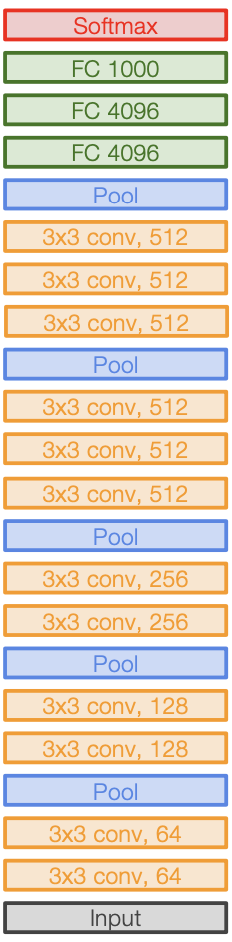
\includegraphics[height=0.7\textwidth]{img/vgg16.png}
	\caption{VGG16 Architecture}
	\label{fig:vgg16}
\end{figure}

\subsubsection{Test 1: Classical VGG16 (Feature Extraction)}
The original VGG16 comes with a couple of 4096 FC layers followed by 1000 softmax neurons, which is alright for ImageNet but definitely oversized for our purpose. Hence, the convolutional base is left as it is, and the fully-connected block is replaced by the a shrunk version with only 256 neurons per layer, followed by our prediction layer made of 11 neurons\ref{fig:vgg16fe1}.

\begin{figure}[H]
	\centering
	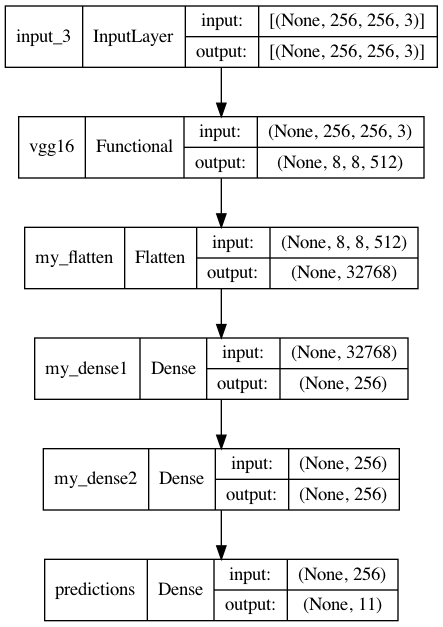
\includegraphics[height=0.5\textwidth]{img/vgg16fe1.png}
	\caption{Our Feature Extraction Network}
	\label{fig:vgg16fe1}
\end{figure}


\noindent The result obtained, using RMSprop as optimizer, are:

\medskip

\begin{tabular}{ |p{2cm}|p{2cm}|p{2cm}|p{2cm}|p{2cm}|  }
\hline
\multicolumn{5}{|c|}{Feature Extraction} \\
\hline
\textbf{Epoch stopped} & \textbf{Validation Accuracy} & \textbf{Testing Accuracy} & \textbf{Validation Loss} & \textbf{Testing Loss} \\
\hline
12 & 0.7409 & 0.7057 & 5.1959 & 5.7\\
\hline
\end{tabular}

\medskip

 \noindent The network begin to overfit very fast, hence some regularization methods are needed.


\begin{figure}[H]
	\centering
	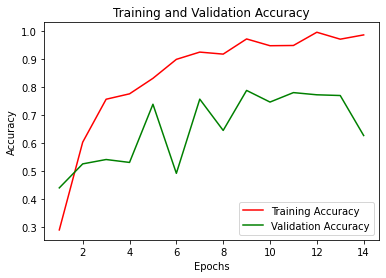
\includegraphics[height=0.45\textwidth]{img/vgg16fe1acc.png}
	\caption{Our Feature Extraction Network Accuracy}
	\label{fig:vgg16fe1acc}
\end{figure}

\begin{figure}[H]
	\centering
	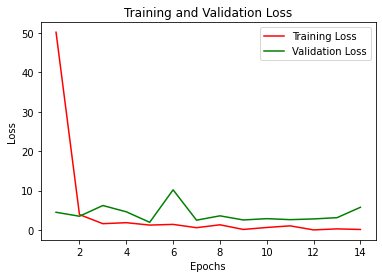
\includegraphics[height=0.45\textwidth]{img/vgg16fe1loss.png}
	\caption{Our Feature Extraction Network Loss}
	\label{fig:vgg16fe1loss}
\end{figure}

\subsubsection{Test 2: Adding dropout to Test 1}
We have two possible positions to use the dropout layer in our network and they are after each 256-dense layer, thus we change our previous network in the following way\footnote{We didn't use a dropout layer between the two 256-dense layers, since this type of architecture led to worst performance}:
\begin{figure}[H]
	\centering
	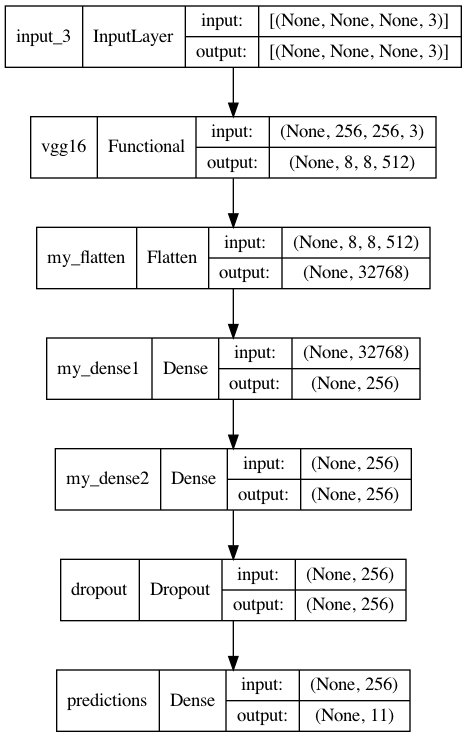
\includegraphics[height=0.45\textwidth]{img/vgg16fe2.png}
	\caption{Our Feature Extraction Network + Dropout}
	\label{fig:vgg16fe2}
\end{figure}
  

\noindent The result obtained, using RMSprop as optimizer, are:

\medskip

\begin{tabular}{ |p{2cm}|p{2cm}|p{2cm}|p{2cm}|p{2cm}|  }
\hline
\multicolumn{5}{|c|}{Feature Extraction} \\
\hline
\textbf{Epoch stopped} & \textbf{Validation Accuracy} & \textbf{Testing Accuracy} & \textbf{Validation Loss} & \textbf{Testing Loss} \\
\hline
25 & 0.7306 & 0.7195 & 3.0616 & 3.0035\\
\hline
\end{tabular}

\medskip

\begin{figure}[H]
	\centering
	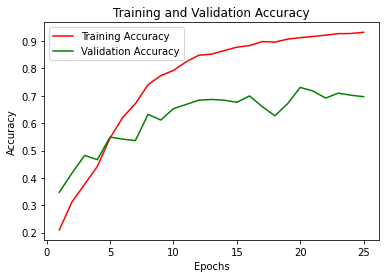
\includegraphics[height=0.45\textwidth]{img/vgg16fe2acc.png}
	\caption{Our Feature Extraction Network Accuracy}
	\label{fig:vgg16fe2acc}
\end{figure}

\begin{figure}[H]
	\centering
	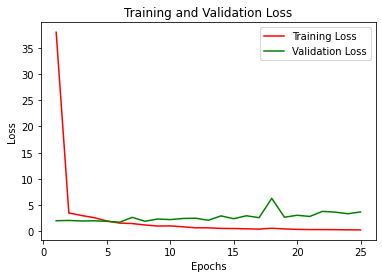
\includegraphics[height=0.45\textwidth]{img/vgg16fe2loss.png}
	\caption{Our Feature Extraction Network Loss}
	\label{fig:vgg16fe2oss}
\end{figure}

\noindent TODO: As expected, dropout mitigated the magnitude of overfitting, now the networks need more time to reach high values of training accuracy and the validation improved to ???.



\subsubsection{Test 3: Fine Tuning One Convolutional Layer}
Using the model defined in test 1, the 3rd Conv2D layer in the 5th block is un-fronzen and the network is trained. The result obtained using RMSprop as optimizer are the following:

 
 \medskip

\begin{tabular}{ |p{2cm}|p{2cm}|p{2cm}|p{2cm}|p{2cm}|  }
\hline
\multicolumn{5}{|c|}{Feature Extraction} \\
\hline
\textbf{Epoch stopped} & \textbf{Validation Accuracy} & \textbf{Testing Accuracy} & \textbf{Validation Loss} & \textbf{Testing Loss} \\
\hline
28 & 0.7202 & 0.6253 & 2.3687 & 8.1807\\
\hline
\end{tabular}

\medskip

\begin{figure}[H]
	\centering
	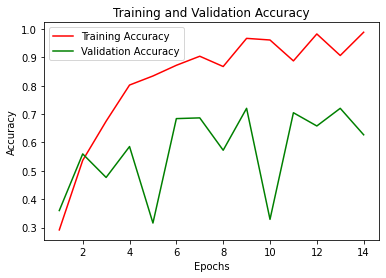
\includegraphics[height=0.45\textwidth]{img/vgg16ft1acc.png}
	\caption{Our Feature Extraction Network Accuracy}
	\label{fig:vgg16ft1acc}
\end{figure}

\begin{figure}[H]
	\centering
	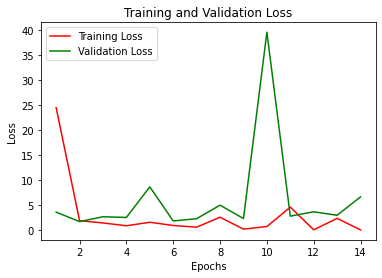
\includegraphics[height=0.45\textwidth]{img/vgg16ft1loss.png}
	\caption{Our Feature Extraction Network Loss}
	\label{fig:vgg16ft1loss}
\end{figure}










\subsubsection{Test 4: test 3 with dropout and different optimizer}
TODO:Using the model defined in test 3, the 3rd Conv2D layer in the 5th block is un-fronzen and the network is trained. The result obtained using Adam 0.0001 as optimizer are the following:

 
 \medskip

\begin{tabular}{ |p{2cm}|p{2cm}|p{2cm}|p{2cm}|p{2cm}|  }
\hline
\multicolumn{5}{|c|}{Feature Extraction} \\
\hline
\textbf{Epoch stopped} & \textbf{Validation Accuracy} & \textbf{Testing Accuracy} & \textbf{Validation Loss} & \textbf{Testing Loss} \\
\hline
28 & 0.7358 & 0.7218 & 0.9871 & 1.1792\\
\hline
\end{tabular}

\medskip

\begin{figure}[H]
	\centering
	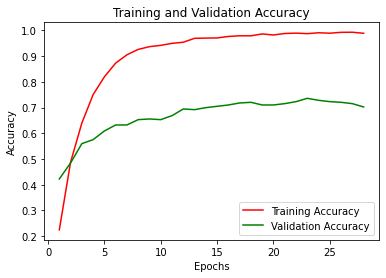
\includegraphics[height=0.45\textwidth]{img/vgg16ft1dropacc.png}
	\caption{Our Feature Extraction Network Accuracy}
	\label{fig:vgg16ft1dropacc}
\end{figure}

\begin{figure}[H]
	\centering
	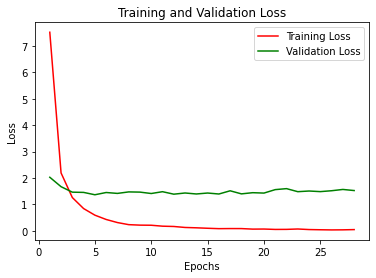
\includegraphics[height=0.45\textwidth]{img/vgg16ft1droploss.png}
	\caption{Our Feature Extraction Network Loss}
	\label{fig:vgg16ft1droploss}
\end{figure}





\subsubsection{Test 5: Fine Tuning Two Convolutional Layers}
Using 4 but with 2 CNN un-frozen

 \medskip

\begin{tabular}{ |p{2cm}|p{2cm}|p{2cm}|p{2cm}|p{2cm}|  }
\hline
\multicolumn{5}{|c|}{Feature Extraction} \\
\hline
\textbf{Epoch stopped} & \textbf{Validation Accuracy} & \textbf{Testing Accuracy} & \textbf{Validation Loss} & \textbf{Testing Loss} \\
\hline
22 & 0.7280 & 0.7379 & 1.4253 & 1.2589\\
\hline
\end{tabular}

\medskip

\begin{figure}[H]
	\centering
	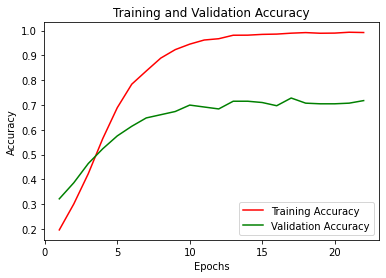
\includegraphics[height=0.45\textwidth]{img/vgg16ft2dropacc.png}
	\caption{Our Feature Extraction Network Accuracy}
	\label{fig:vgg16ft2dropacc}
\end{figure}

\begin{figure}[H]
	\centering
	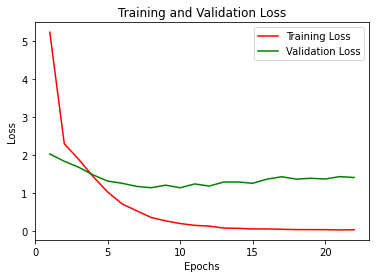
\includegraphics[height=0.45\textwidth]{img/vgg16ft2droploss.png}
	\caption{Our Feature Extraction Network Loss}
	\label{fig:vgg16ft2droploss}
\end{figure}








\subsubsection{Test 6: Fine Tuning One Convolutional Layer + weights regularization}
Using 4 but with 1 CNN un-frozen + L1\_L2



\medskip

\begin{tabular}{ |p{2cm}|p{2cm}|p{2cm}|p{2cm}|p{2cm}|  }
\hline
\multicolumn{5}{|c|}{Feature Extraction} \\
\hline
\textbf{Epoch stopped} & \textbf{Validation Accuracy} & \textbf{Testing Accuracy} & \textbf{Validation Loss} & \textbf{Testing Loss} \\
\hline
22& 0.7487 & 0.7471 & 21.5590 & 9.8097\\
\hline
\end{tabular}

\medskip

\begin{figure}[H]
	\centering
	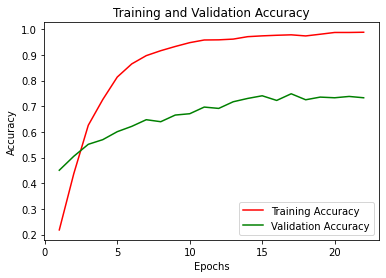
\includegraphics[height=0.45\textwidth]{img/vgg16ft1dropregacc.png}
	\caption{Our Feature Extraction Network Accuracy}
	\label{fig:vgg16ft1dropregacc}
\end{figure}

\begin{figure}[H]
	\centering
	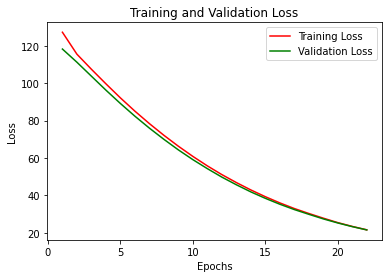
\includegraphics[height=0.45\textwidth]{img/vgg16ft1dropregloss.png}
	\caption{Our Feature Extraction Network Loss}
	\label{fig:vgg16ft1dropregloss}
\end{figure}









\subsubsection{Test 7: Fine Tuning Two Convolutional Layers + weights regularization}
Using 5 but with 2 CNN un-frozen + L1\_L2

 \medskip

\begin{tabular}{ |p{2cm}|p{2cm}|p{2cm}|p{2cm}|p{2cm}|  }
\hline
\multicolumn{5}{|c|}{Feature Extraction} \\
\hline
\textbf{Epoch stopped} & \textbf{Validation Accuracy} & \textbf{Testing Accuracy} & \textbf{Validation Loss} & \textbf{Testing Loss} \\
\hline
25 & 0.7694 & 0.7494 & 15.6742 & 9.8097\\
\hline
\end{tabular}

\medskip

\begin{figure}[H]
	\centering
	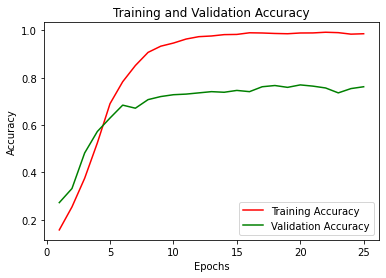
\includegraphics[height=0.45\textwidth]{img/vgg16ft2dropregacc.png}
	\caption{Our Feature Extraction Network Accuracy}
	\label{fig:vgg16ft2dropregacc}
\end{figure}

\begin{figure}[H]
	\centering
	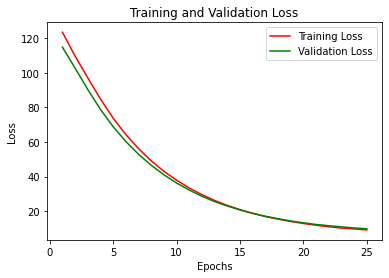
\includegraphics[height=0.45\textwidth]{img/vgg16ft2dropregloss.png}
	\caption{Our Feature Extraction Network Loss}
	\label{fig:vgg16ft2dropregloss}
\end{figure}









\subsubsection{Test 8: Genetic Algorithm for Hyper-parameters and Architecture Optimization}





\subsection{ResNet50V2}

\subsubsection{Test 1: Classical ResNet50V2 (Feature Extraction)}
On a small dataset, overfitting will be the main issue. Data augmentation is a powerful way to fight overfitting when you’re working with image data.

\subsubsection{Test 2: Completely New Output Layers Architecture}

\subsubsection{Test 3: 1 and 2 with Data Augmentation}

\subsubsection{Test 4: Fine Tuning with One Layer}

\subsubsection{Test 5: Fine Tuning with Two Layers}







\subsection{ResNet101V2}

\subsubsection{Test 1: Classical ResNet101V2 with 50 classes}

\subsubsection{Test 2: Completely Newly Output Layers Architecture}

\subsubsection{Test 3: Fine Tuning with One Layer}

\subsubsection{Test 4: Fine Tuning with Two Layers}







\subsection{InceptionV3}

\subsubsection{Test 1: Classical ResNet101V2 with 50 classes}

\subsubsection{Test 2: Completely Newly Output Layers Architecture}

\subsubsection{Test 3: Fine Tuning with One Layer}

\subsubsection{Test 4: Fine Tuning with Two Layers}
